\section{Įvadas}

Su kompiuterinės grafikos vizualizacijomis dirbančios specialiųjų efektų
studijos jau gana seniai pastebėjo, kad kai kuriems efektams (Pavyzdžiui:
rūko, debesų, sprogimų) išgauti poligoninių paviršių vizualizavimas nėra
geriausia išeitis. Ypač jeigu norima pasieki detalų, stambiam planui tinkantį
rezultatą. Tūriniams efektams vizualizuoti dažniausiai pasitelkiamos tūrinių
objektų vizualizavimo technikos, žinomos bendriniu „vokselių vizualizavimo
technologijų“ pavadinimu.

Vokselių vizualizavimas taip pat naudojamas įvairiuose moksliniuose
įrankiuose, kur būtina vaizduoti „neoptimizuotus“ (nepakeistus) tūrinius
objektus (Pavyzdžiui, medicinos tyrimai).

Prieš tai minimi atvejai nėra iš realaus laiko 3D vaizdavimo srities. O
pastarojoje tūrinis vizualizavimas yra ganėtinai apleista sritis. Tą sąlygojo
techninės galimybės. Tačiau dabar aparatūrinė įranga jau įgalina vaizduoti
tūrinius objektus realiu laiku. Būtent šiai sričiai -- tūrinių objektų realaus
laiko vizualizacijai -- šiame darbe yra skiriamas didžiausias dėmesys. Jame
yra pristatomas autoriaus sukurtas realaus laiko vokselių vizualizavimo ir
normavimo įrankis.

Darbo tikslai:

\begin{itemize}
\item Pristatyti vokselių idėją
\item Pristatyti pagrindines tūrinių objektų vaizdavimo koncepcijas
\item Pristatyti sukurtą realaus laiko vokselių vizualizavimo ir
normavimo įrankį
  \begin{itemize}
  \item Apžvelgti transformavimo filtrą
  \item Apžvelgti globalaus permatomumo filtrą
  \item Apžvelgti apšvietimo sustiprinimo filtrą
  \end{itemize}
\end{itemize}

\begin{figure}[b]
\centering
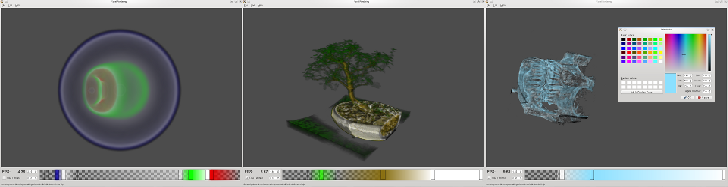
\includegraphics[width=16.5cm]{teaser.png}
\caption{Darbe pristatomas vokselių vizualizavimo ir normavimo įrankis.}
\label{fig:teaser}
\end{figure}

